\chapter{Marco Teórico}

La marea se divide en dos componentes principales: marea astronómica y marea meteorológica (Fig \ref{fig:mareas}). 

\begin{figure}
	\centering
	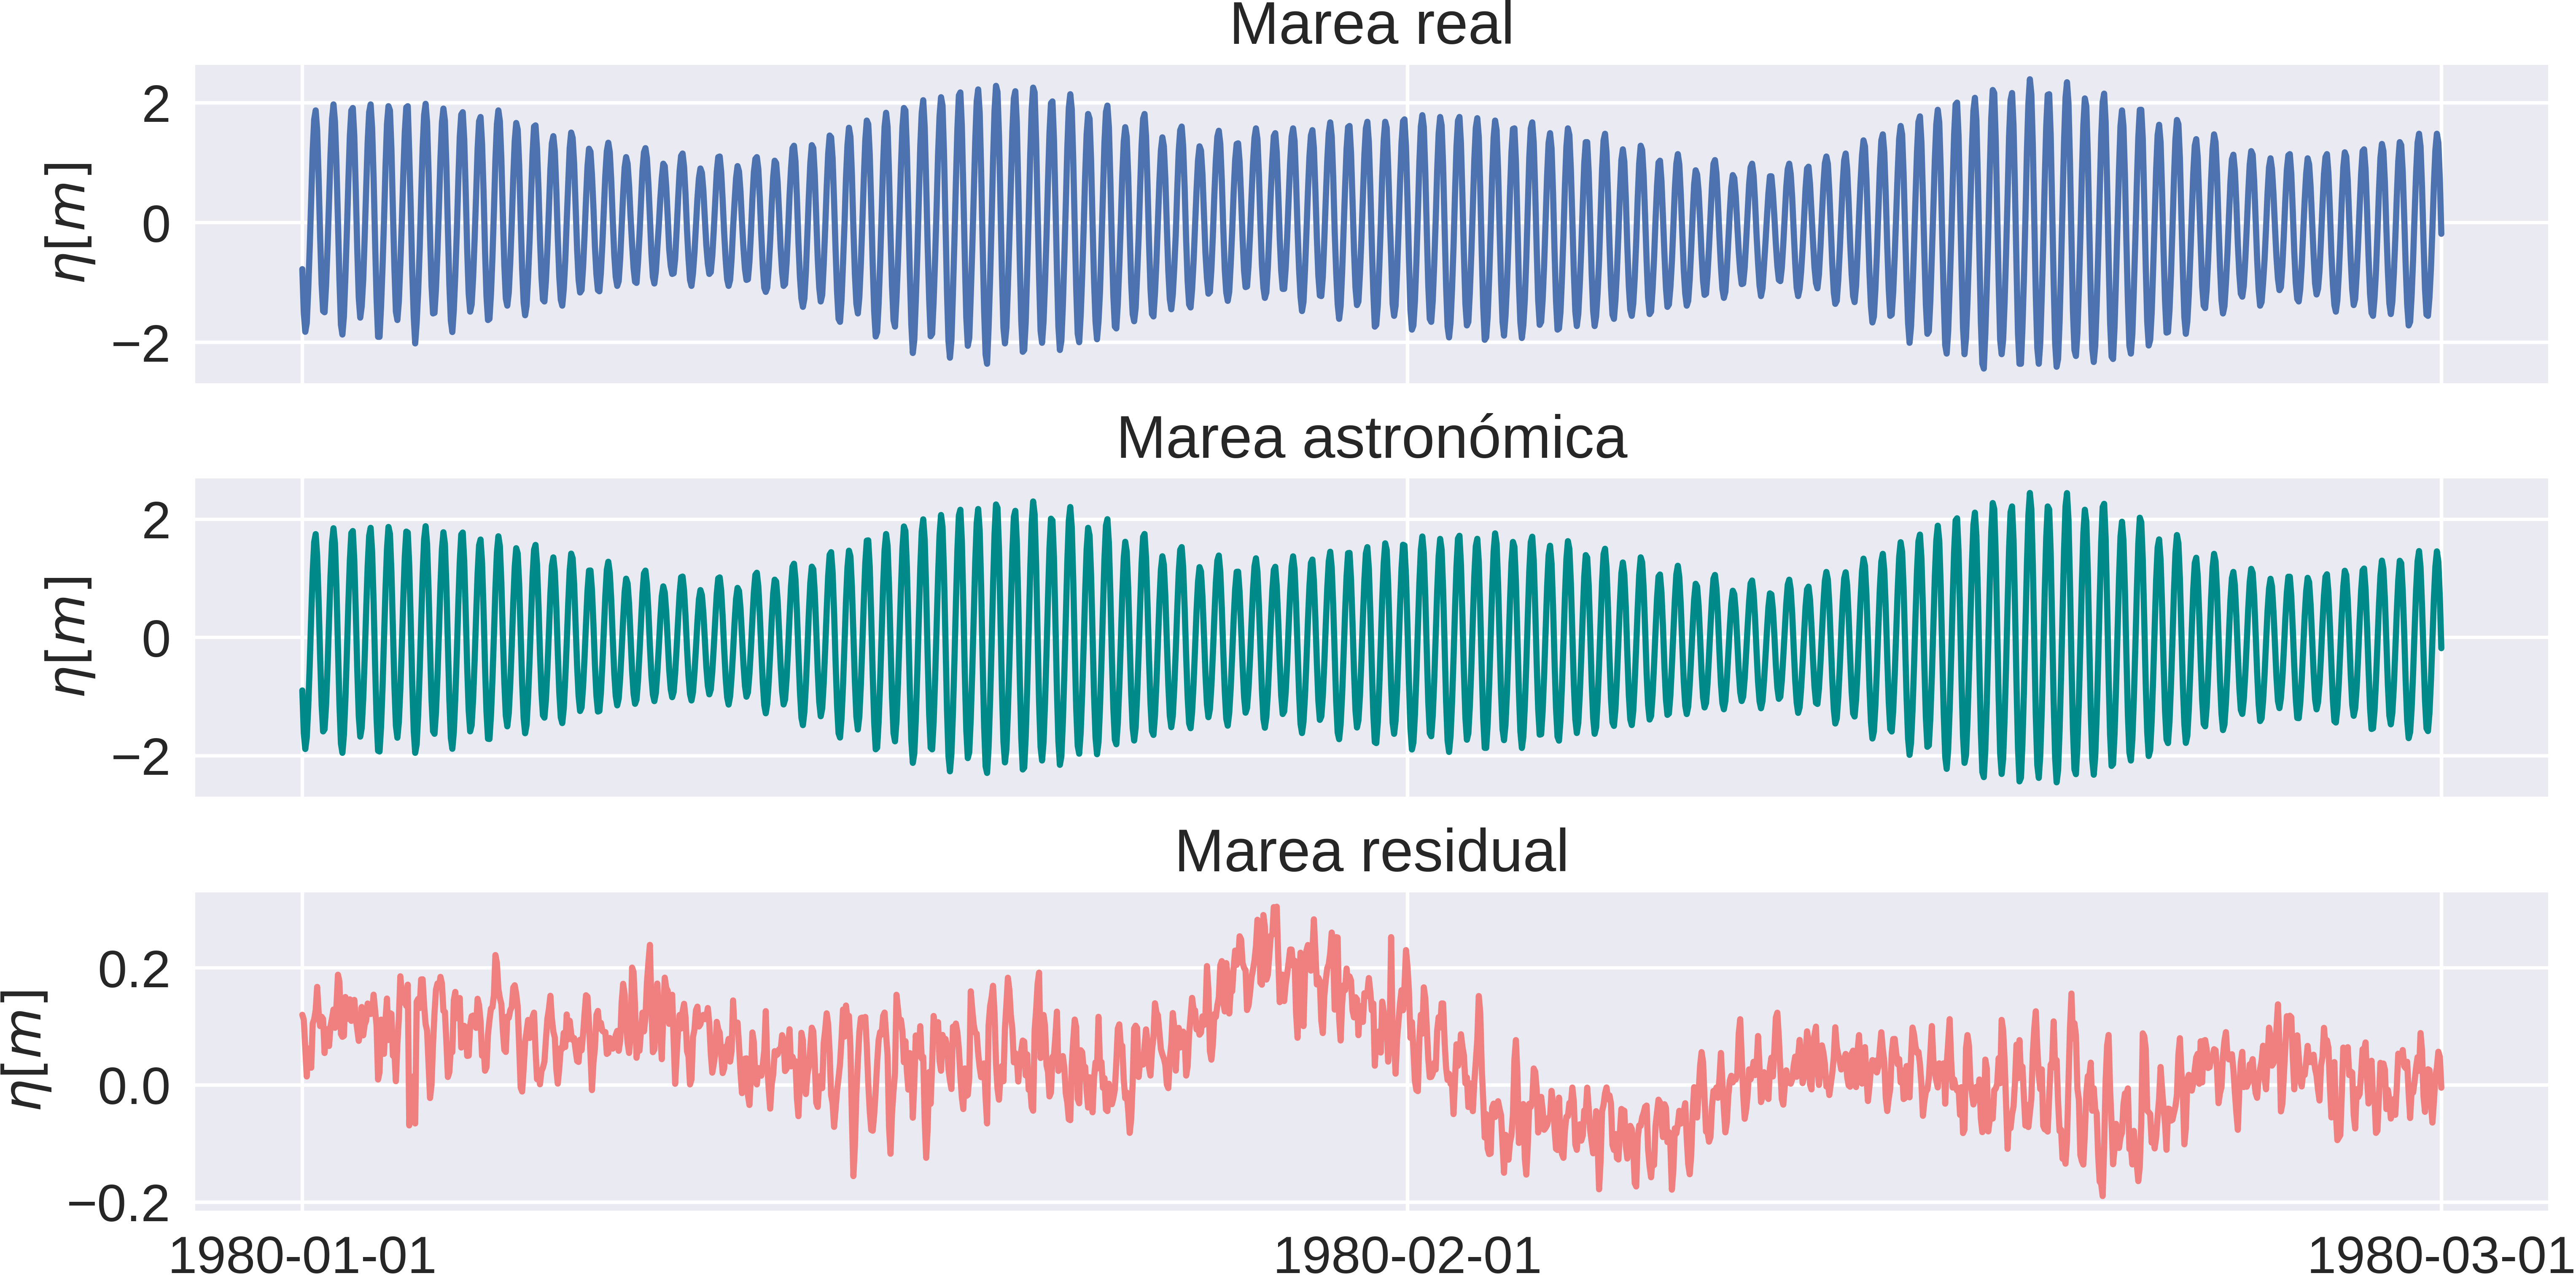
\includegraphics[scale=0.6]{series_marea.png}
	\caption{Series de marea y sus componentes para un período de ejemplo.}
	\label{fig:mareas}
\end{figure}


\section{Marea astronómica}

La marea astronómica se define como el desbalance entre la atracción gravitatoria y la fuerza
centrífuga en el sistema Tierra-Sol-Luna. La resultante entre estas dos fuerzas se llama fuerza generadora de marea y su componente en x se define como la fuerza tractora que origina la marea (su componente en y es despreciable respecto a la gravedad). A continuación se presenta la fórmula que describe esta fuerza contemplando sólo el sistema tierra-luna:

\begin{equation}F_{t}=\frac{3}{2} G M_{L} \frac{R_{t}}{R^{3}} \sin 2 \theta\end{equation}

Donde la G representa la constante de atracción gravitatoria entre la tierra y la luna, $M_{L}$ es la masa de la luna, $R_{T}$ es el radio de la tierra y R es la distancia entre los centros de gravedad de la tierra y la luna.

El estudio de la marea astronómica se puede realizar a través de diferentes técnicas: a) teoría general de equilibrio propuesta por Isaac Newton, b) teoría dinámica basada en la resolución de las ecuaciones fundamentales de la hidrodinámica \citep{Jesus2005} y c) análisis armónico fundamentada en la descomposición armónica \citep{Dronkers1975}, \citep{Schuremann1958}.

La teoría general de equilibrio es útil para el entendimiento cualitativo de la marea astronómica, más que para la determinación precisa de sus características determinantes, específicamente su amplitud y su fase, dado que asume ciertas hipótesis como que los océanos cubren la superficie terrestre completamente, de tal forma
que las partículas de agua se moverán hasta a alcanzar una superficie de
equilibrio y que la respuesta de la capa de agua es instantánea (se desprecia la inercia). Sin embargo, los efectos de contorno y las fuerzas inerciales sí tienen una gran importancia en la determinación de la marea.

La teoría dinámica emplea las ecuaciones de Navier-Stokes  simplificadas para la determinación de las variaciones en la superficie libre del flujo y la propagación de la onda de marea. Dichas ecuaciones toman en cuenta la interacción de dichas ondas con fondos someros o con contornos geográficos y estiman bien las magnitudes de la amplitud, la fase y los períodos, sin embargo requieren de mucha información para la calibración de los modelos que las solucionan.

El análisis armónico descompone la señal de marea en un número finito de señales (componentes armónicas) que tienen una amplitud, período y fase correspondiente y que están previamente definidos por su relación directa con los movimientos astronómicos relativos entre la tierra, la luna y el sol.

\begin{equation}
\eta (t)=a_{0}+\sum_{t=1}^{n} a_{i} \cos \left(\varpi t+\varphi_{i}\right)
\end{equation}

donde, 

$a_{0}$ es la amplitud del nivel medio de referencia\\
$a_{i}$ es la amplitud de la onda i\\
$\omega_{i}$ es la frecuencia de la onda componente i\\
$\phi_{i}$ es el desfase de la onda componente i\\
t es el instante en que se calcula la marea\\
n es el número de componentes consideradas\\

Existen herramientas computacionales que realizan la descomposición armónica de la marea, algunas de estas están estructuradas en MATLAB o Python \citep{Pawlowicz2002} y para su implementación correcta no pueden existir muchos vacíos en los registros de marea, puesto que se distorsionan los cálculos de las amplitudes. La descomposición armónica bajo el uso de la herramienta PyTides es más eficaz puesto que usa las fechas de los registros existentes para la interpolación de los datos faltantes. Los cinco armónicos que más aportan a la componente astronómica de la marea en Buenaventura, en términos de la amplitud, se presentan a continuación.

\begin{table}[H]
	\centering
	\begin{tabular}{|c|c|}
		\hline
		Componente & Amplitud [m] \\
		\hline
		M2      &  1.496 \\
		S2      &  0.421 \\
		N2      &  0.314 \\
		K1      &  0.115 \\
		K2      &  0.104 \\
		\hline
	\end{tabular}
	\caption{Principales 5 componentes de la marea astronómica}
	\label{table:componentes}
\end{table}

Según la tabla \ref{table:componentes}, las principales componentes son: principal lunar ($M_{2}$), principal solar ($S_{2}$), principal elíptica ($N_{2}$), principal menor ($K_{2})$ y principal medio-mayor ($K_{1}$). Estas componentes y sus repectivos valores de amplitud son congruentes con los reportados en estudios anteriores \citep{Malikov2010}. La marea es de tipo \textbf{semidiurna} \citep{MolaresBabra2004}, según el coeficiente de Coutier (eq. \ref{eqn:coutier}) usado para la clasificación de la marea.

\begin{equation}
F=\frac{ K_{1}-O_{1}}{M_{2}-S_{2}}
\label{eqn:coutier}
\end{equation}

La marea astronómica es afectada por diferentes fenómenos, la traslación de la luna alrededor de la tierra que genera la duracion de un día lunar mayor al día solar, la declinación de la luna respecto a la tierra, debido a que la luna no está en el plano del ecuador, sino que se encuentra declinada entre 18.5\textdegree 28.5\textdegree, dicha variación marca el ciclo nodal de la luna y se repite cada 18.61 años, el efecto de las órbitas elípticas amplifica los valores de marea durante el perigeo y el perihelio y la acción conjunta del sistema Tierra-Sol-Luna que genera los períodos de marea viva o de sicigia, cuando la alineación del sol, la tierra y la luna genera la mayor fuerza de atracción y por ende, hay pleamares mayores al promedio y bajamares menores al promedio, de igual forma se perciben los períodos de marea muerta o de cuadratura dónde sucede lo contrario; pueden notarse en la marea astronómica de la figura \ref{fig:mareas} dónde se presenta una intensificación de las aumentos y descensos del nivel en períodos de aproximadamente 15 días, adicionalmente aparece la diferencia entre la pleamar y la bajamar llamada carrera de marea, y su valor es aproximadamente 4 metros.

\section{Marea meteorológica}

Por otro lado, la marea meteorológica se debe a la acción de fenómenos que inducen, tensiones tangenciales en el nivel del mar que pueden converger y por lo tanto, generar un ascenso del nivel del mar como de variaciones en la fuerza vertical que la presión atmosférica ejerce sobre la superficie del mar. Esta marea se puede representar como los residuos meteorológicos en la serie después de eliminar los componentes armónicos de la marea. Los residuos son de carácter, por lo que es difícil su predicción.

La serie residual de la marea (panel superior en la fig \ref{fig:sobre}) es la serie de interés en este estudio, puesto que es la componente que está condicionada por fenómenos meteorológicos. Se llamará de aquí en adelante \textbf{serie de nivel del mar} y dada su resolución, es posible determinar tres series a partir de ella con una resolución menor que permitan entender análisis posteriores.

\begin{enumerate}
	\item Serie mensual de nivel del mar: Obtenida a partir del promedio mes a mes de la serie de nivel del mar en resolución horaria.
	\item Series de sobrelevaciones y descensos diarios de nivel del mar: Obtenidas a partir de los máximas sobrelevaciones y descensos del nivel que ocurren en un día (panel inferior en la fig \ref{fig:sobre})
	\item Series de sobrelevaciones y descensos mensuales del nivel del mar: Obtenidas a partir de la media mensual de las series de sobrelevaciones y descensos diarios.
\end{enumerate}

La última serie se calcula porque debe distinguirse que un valor medio mensual del nivel desde el registro horario será menor a un valor medio mensual desde el registro de máximos diarios. Estos última serie brinda información más fidedigna que lo que registró el mareografo. 

\begin{figure}[h]
	\centering
	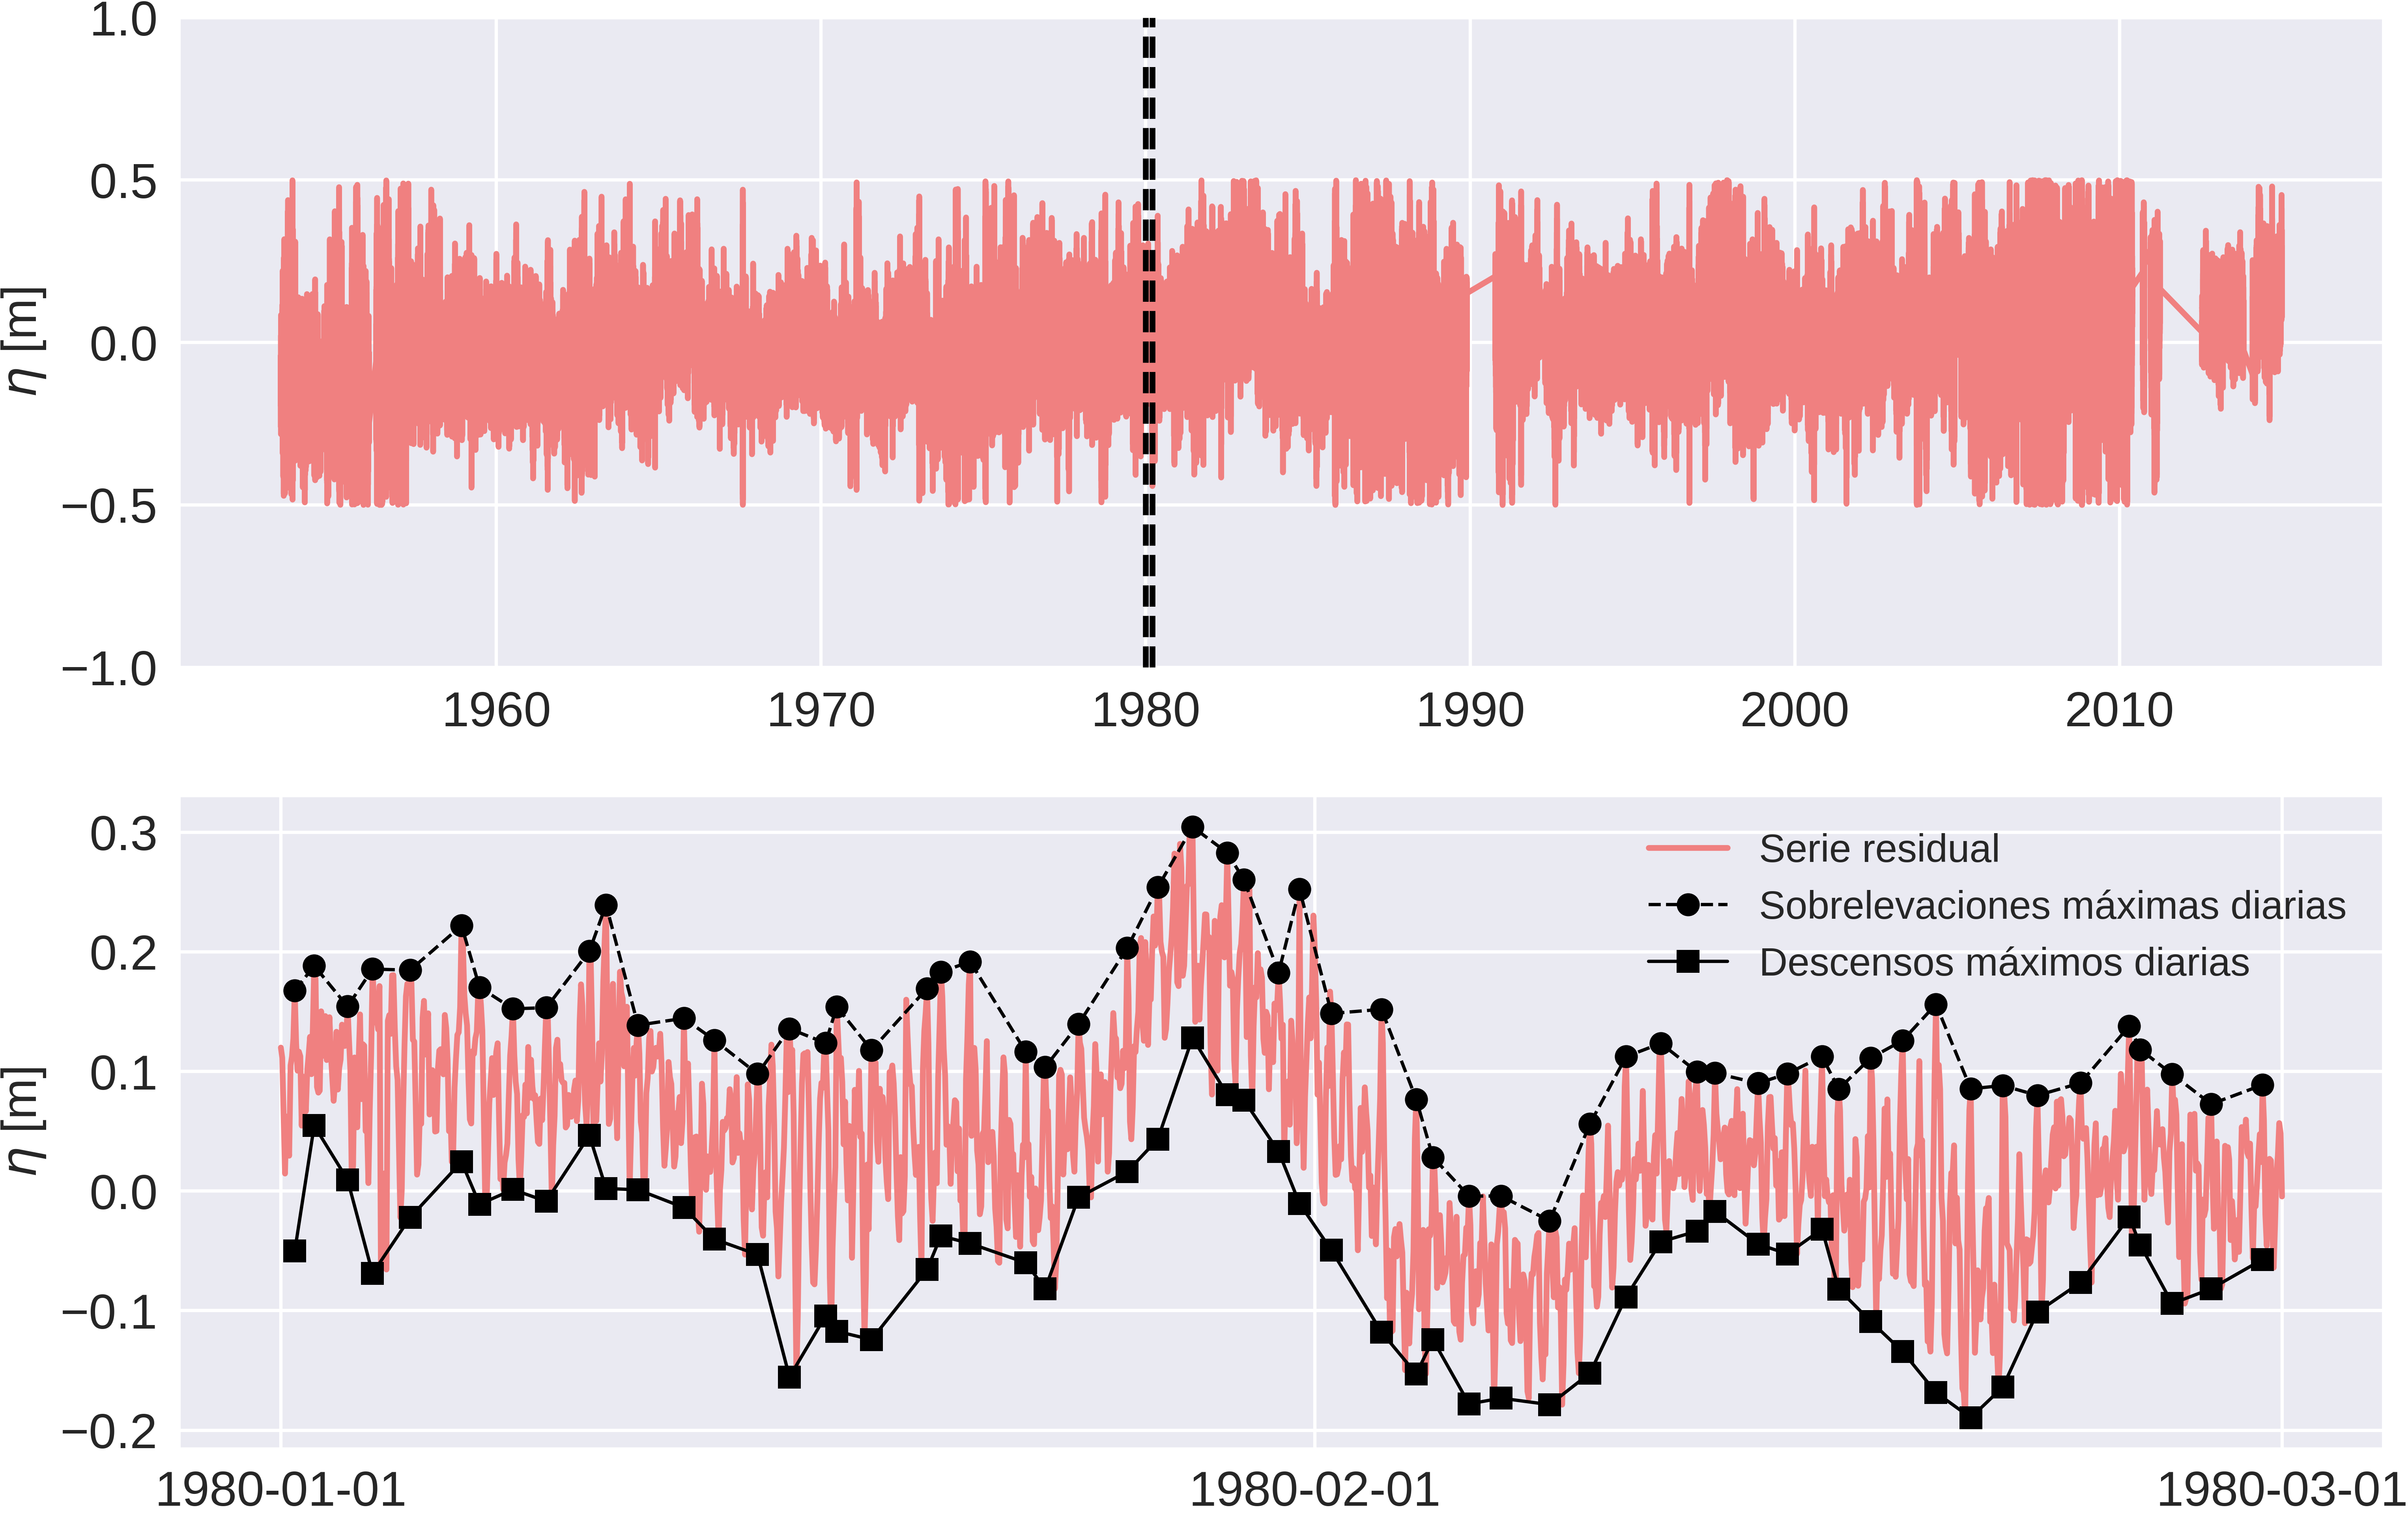
\includegraphics[scale=0.6]{sobrelevaciones_maximas.png}
	\caption{Series de sobrelevaciones y descensos máximos diarios del nivel del mar}
	\label{fig:sobre}
\end{figure}

\section{Análisis descriptivo de la variación del nivel del mar}

Una serie temporal de alguna variable se puede descomponer en una parte estacional ($E_{t}$), una parte de tendencia $T_{t}$ y una parte asociada a ruido $R_{t}$ (eq \ref{eqn:serie est}). La componente de ruido se debe a la aleatoriedad de la variable y su carácter no es determinista, sin embargo, las otras dos componentes si lo son. 

\begin{equation}
X_{t}=E_{t}+I_{t}+R_{t}
\label{eqn:serie est}
\end{equation}

Ciertas técnicas de análisis de datos requieren que la información sea estacionaria, por lo tanto, se debe suprimir la tendencia que pueda tener el registro. La estimación de la tendencia se puede realizar desde un enfoque determinista o evolutivo, según la naturaleza de la serie.

\subsection*{Nivel medio del mar}

Todos los estudios del nivel del mar en una región local no 
utilizan la información de altura de nivel sobre un datum de referencia global, sino que determinan un nivel medio del mar relativo a la zona y es calculado como el valor medio del registro, así, todos los valores que estén por encima del nivel medio del mar local se llaman \textbf{sobrelevaciones} y por debajo del nivel del mar \textbf{descensos}.

La información del nivel del mar se suaviza realizando medias en ventanas móviles de tamaños específicados, para comparaciones se realizan con un tamaño de 3 meses y así, la variación trimestral queda suprimida de la serie. El suavizado de un registro es similar en ciertas características al filtrado en alguna banda espectral de interés.

La caracterización de las distribuciones de sobrelevaciones máximas y descensos máximos durante los eventos Niño y Niña se determina con un diagrama de caja y bigotes que muestre los rango intercuartílicos y los percentiles 25, 50 y 75. En términos espaciales, un tipo de gráfica útil es el diagrama de Hövmoller, en él, se determinan los cambios de alguna variable respecto a una longitud o una latitud.


\section{Análisis espectral}

Un proceso físico puede ser descrito en el dominio
del tiempo con una función $f(t) $ dónde la variable toma un valor específico en un momento diferente. Expresar una función en estos términos no puede dar mucho información de los fenómenos que la afectan cuando el registro de la variable es muy largo y su variabilidad es alta, por lo tanto, es posible utilizar el dominio de la  frecuencia, en donde el fenómeno de interés puede ser descrito por su amplitud y fase en función de la frecuencia (Fig. \ref{fig:a_e})

\begin{figure}
	\centering
	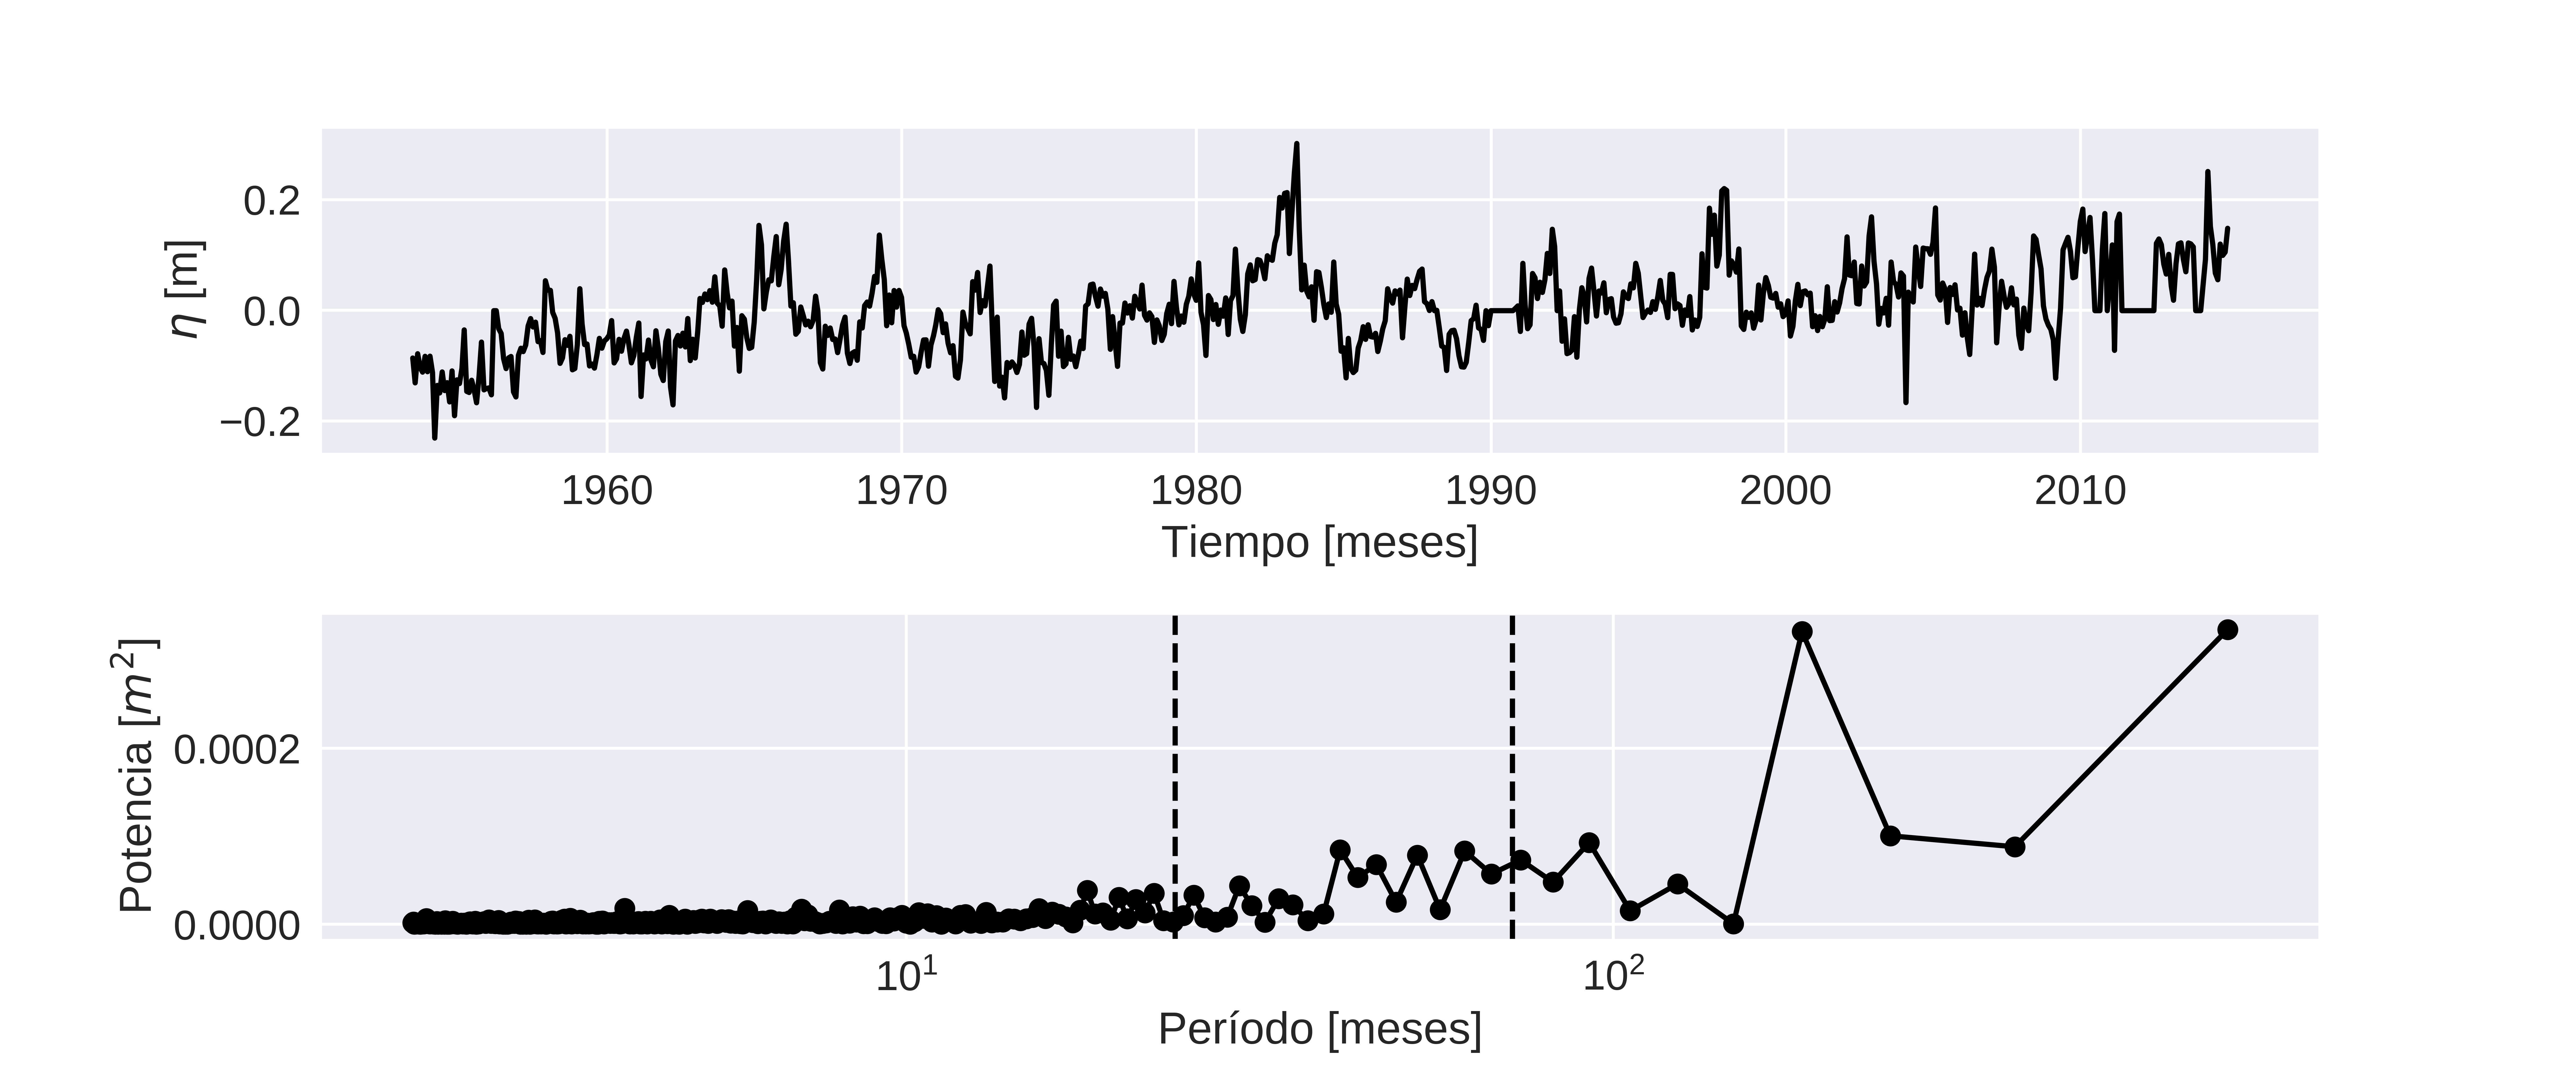
\includegraphics[scale=0.6]{Espectro.png}
	\caption{Serie en el dominio temporal y en el dominio espectral}
	\label{fig:a_e}
\end{figure}

Dada la aleatoriedad de la serie meteorológica del nivel del mar, es más efectivo descomponer esta señal en frecuencias diferentes y comprender los fenómenos climáticos que pueden asociarse a cada una de ellas. Un método ampliamente usado para esta descomposición en el dominio frecuencial es la transformada de Fourier. Esta transformación matemática es el mapeo del conjunto de series sumables que componen una serie \citep{Lund2000}, si \textit{s} es una serie sumable de este conjunto con una frecuencia $\omega$, su transformada $\mathcal{F}\{s\}$ se define como:

\begin{equation}
\mathcal{F}\{s\}(\omega)=\sum_{j=-\infty}^{\infty} s_{j} e^{-i 2 \pi \omega j}
\label{eqn:normal}
\end{equation}

El término $e^{-i 2 \pi \omega j}$ puede escribirse como un conjunto de ondas sinusoidales de la forma, $\cos (2 \pi \omega j)-i \cdot \operatorname{sen}(2 \pi \omega j)$. Es entonces evidente, que el método hace corresponder una serie con una sumatoria de ondas. 

Esta transformada a partir de una secuencia y con una duración finita se conoce mejor como Transformada Discreta de Fourier (DFT por sus siglas en inglés), pero su rendimiento puede verse potenciado cuando se reduce el tiempo de cálculo de $n^{2}$ pasos a $n \cdot log_{2}(n)$ pasos
al aplicarse en subsucesiones más cortas. Este mejoramiento se convierte en la Transformada Rápida de Fourier (FFT por sus siglas en inglés) 

Una de las propiedades más importantes de la transformada de Fourier es la posibilidad de invertirse para cambiarse del dominio de la frecuencia al dominio del tiempo, esta aplicación es muy útil cuando desea conocerse el comportamiento de la variable bajo ciertas frecuencias de interés. Esta función es la transformada de Fourier inversa \ref{eqn:inversa} y su uso es amplio de el estudio de variables oceánicas en escalas mayores al año.

\begin{equation}
s_{j}=\int_{-\frac{1}{2}}^{\frac{1}{2}} \mathcal{F}\{s\}(\omega) e^{i 2 \pi \omega j} d \omega
\label{eqn:inversa}
\end{equation}

En este caso cada componente j-ésima de la serie mensual de nivel del mar se obtiene integrando el espectro de potencias de Fourier en su respectiva frecuencia ($\omega$) 

Otra propiedad útil de la transformada de Fourier es que la sumatoria total de las potencias del espectro representan la varianza total de la serie, esto es sumamente útil para la realización de los mapas de varianza de las variables espaciales que se vayan a analizar.

Con las variables espaciales se pueden construir funciones ortogonales empíricas que permitan explorar la estructura de su variabilidad de forma objetiva y analizar relaciones con otras variables.

\section{Análisis de componentes principales}

El objetivo de un análisis de componentes principales (ACP) es la determinación de un conjunto de funciones ortogonales empíricas que permitan la representación de un conjunto de datos X(x,y,t) en:

\begin{equation}
X(x, y, t)=\sum_{i=1}^{M} P C_{i}(t) \cdot E O F_{i}(x, y)
\end{equation}

Donde: \\
- $PC_{i}$ es la componente principal i-ésima que determinan la variación de la estrucutra espacial en el tiempo y es ortogonal a otras PC's en el tiempo.\\
- $EOF_{i}$ es una estructura espacial obtenida a partir de los vectores propios de la matriz de covarianza y en este caso, es ortogonal en el espacio a otras EOF's.

Cada una de las PC's pueden obtenerse a partir de la proyección de la información espacial sobre cada una de las EOF's. Los conceptos de proyección y correlación están íntimamente ligados, puesto que representan el grado de similitud que tiene una información con respecto a otra, así que entre mayor sea la proyección para una PC, mayor va a ser la varianza explicada por ese componente principal. Dado que cada PC y EOF es calculada para maximizar varianza manteniendo ortogonalidad entre ellos y no para tener sentido físico, es de estricto cuidado las conclusiones que se generen a partir de ellas.

La determinación de las EOF se realiza con las matrices de covarianza o correlación. El uso de una o la otra dependerá de las condiciones que se deseen evaluar y de las variables empleadas, a continuación se explican sus diferencias:

\begin{itemize}
	\item Matriz de correlación: Todas las variables tienen igual peso, por lo tanto, sólo importa la estructura espacial (EOF). Su uso se recomienda cuando las variables a emplear tienen diferentes unidades y cuando las varianzas de cada una de las variables difieren mucho entre sí y pueden distorsionar los resultados.
	\item Matriz de covarianza: En las EOF's calculadas con esta matriz se da mas peso a aquellas variables que tienen mayor varianza. Su uso se recomienda cuando se quiere generar una mayor importancia sobre ciertas variables.
\end{itemize}

El cálculo computacional de la EOF, se da desde la matriz tridimensional M (x,y,t) donde para cada tiempo t se tiene un patrón espacial. Posteriormente, se debe realizar una redistribución de los datos de la matriz M a una matriz A con dimensiones (t,x*y) donde en una dimensión está la variación temporal de un píxel y en otra todos la variación píxel a píxel.  

Finalmente, el cálculo de la EOF termina con la factorización de la matriz A:

\begin{equation}
A  = U \cdot S \cdot V^H
\end{equation}

Donde U y V corresponden a los patrones espaciales y temporales obtenidos y S la varianza que aporta cada PC

\section{Medidas de correlación lineal}

Para determinar si la relación lineal existente entre dos variables continua es fuerte o no, se debe disponer de ciertos parámetros que cuantifiquen esta relación. Uno de estos parámetros es la covarianza, que indica el grado de variación conjunta de dos variables aleatorias.

\begin{equation}
\text { Covarianza muestral }=\operatorname{Cov}(X, Y)=\frac{\sum_{i=1}^{n}\left(x_{i}-\bar{x}\right)\left(y_{i}-\bar{y}\right)}{N-1}
\end{equation}

donde $\bar{x}$ y $\bar{y}$ representan las medias muestrales de cada variable y $x_{i}$ e $y_{i}$ los valores para cada una de las observaciones.

Dado que las escalas de las variables que se correlacionen pueden diferir mucho una de la otra, deben escalarse y generar lo que se conoce como coeficiente de correlación. Los valores de estos coeficientes oscilan entre -1 y +1 y entre mayor sea, mayor es la fuerza de la relación lineal proporcional o inversa entre las variables. Un coeficiente de correlación importante es el de Spearman y al ser no paramétrico, no es susceptible a la aparición de outliers.

\section{Red Neuronal Artificial (RNA)}

   Una red neuronal artificial (RNA) se puede definir como un grafo dirigido con las siguientes restricciones \citep{HECHT-NIELSEN1992}:

\begin{enumerate}
	\item Los nodos se llaman elementos de proceso (EP).
	\item Los enlaces se llaman conexiones y funcionan como caminos unidireccionales instantáneos
	\item Cada EP puede tener cualquier número de conexiones.
	\item Todas las conexiones que salgan de un EP deben tener la misma señal.
	\item Los EP pueden tener memoria local.
	\item Cada EP posee una función de transferencia que, en función de las entradas y la memoria local produce una señal de salida y / o altera la memoria local.
	\item Las entradas a la RNA llegan del mundo exterior, mientras que sus salidas son conexiones que abandonan la RNA
\end{enumerate}

\begin{figure}[H]
	\centering
	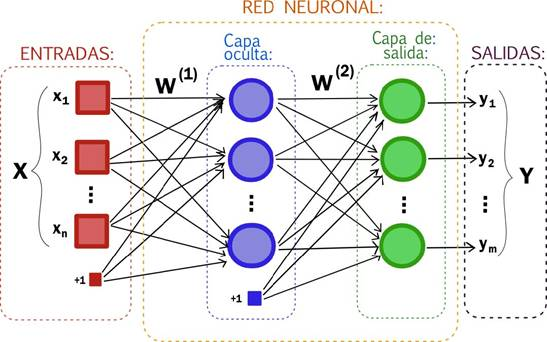
\includegraphics[scale=0.8]{estructura.jpg}
	\caption{Ejemplo de estructura de red neuronal (Tomado de Google Images)}
	\label{fig:e_red}
\end{figure}

Son ampliamente utilizadas para reconocer patrones de comportamiento y realizar modelos de predicción y están conformadas por los siguientes elementos:

\begin{itemize}
	\item Conjunto de vectores de entrada, $x$ o capa de entrada: En esta capa aparece un nodo por cada variable predictora dentro del modelo de la red neuronal. Estas variables predictoras deben ser, en la mayoría de los casos, pre-procesadas para que su peso inicial sobre la red sea igual al de otras variables, esto mejorará el rendimiento. Típicamente se estandarizan y se escalan según la función de activación a emplear.
	\item Conjunto de capas intermedias: también son llamadas capas ocultas y se caracterizan porque no reciben ni suministran información al entorno (procesamiento interno de la red).
	\item Conjunto de pesos sinápticos $w_{ij}$: representan la interacción entre los nodos de las capas de la red neuronal, estos pesos se optimizan continuamente hasta disminuir al máximo el error de la red.
	\item Regla de propagación f($w_{ij}$,$x_{j}(t)$): es la regla que sigue la red para la conjugación de los pesos de la red y los valores de las variables de entrada, una regla ampliamente utilizada es 
	\item Función de activación, k(f($w_{ij}$,$x_{j}(t)$)): proporciona el estado de activación de un nodo de la red neuronal, existen funciones como tangente hiperbólica, sigmoide y lineal. El uso de cada una dependerá de las variables predictoras y a predecir en la red.
	\item Función de salida $F_{i}(t)$: proporciona la salida $y_{i}(t)$, en función del estado de activación.
\end{itemize}
